\documentclass[a4paper,10pt]{article}
\usepackage[left=2cm,top=2cm,right=2cm,bottom=2cm]{geometry}
\usepackage[utf8]{inputenc}
\usepackage{amsthm}
\usepackage{graphicx}
\graphicspath{ {images/} }

\newcommand{\mN}{{\mathbb N}}
\newcommand{\mZ}{{\mathbb Z}}
\newcommand{\cZ}{{\mathcal Z}}
\newcommand{\fL}{{\mathfrak L}}
\newcommand{\dst}{\displaystyle}

%opening
\title{}
\author{}
\date{}

\begin{document}

\maketitle
Carlos Alberto Gallegos Tena \\\\
Tarea 3\\\\
Da un ejemplo, redactado en latex, de una retícula que no sea completa.\\\\
Tomamos la relación dada por el diagrama de Hasse:\\\\
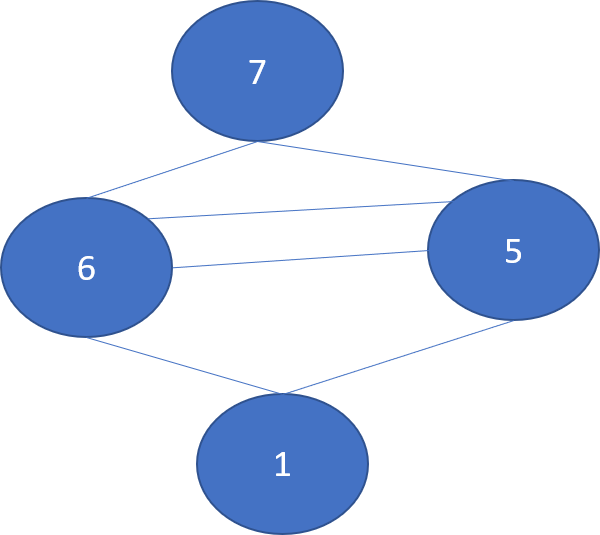
\includegraphics[scale=1]{D2.png}  \\\\
Tomamos el subconjunto $\{6,5\}$,y  nos damos cuenta que no tenemos ninguna mínima cota superior ni máxima cota inferior. Por lo tanto es una retícula no completa.


\end{document}